\newpage

\section{Anexos}

\subsection{Esquemas de conexión}

\subsubsection{Piano electrónico}

En la Figura~\ref{fig:conexion_piano} se muestra el esquema de conexión del piano electrónico, elaborado en Tinkercad®. 
Se pueden observar las conexiones entre el microcontrolador ATmega328P, los pulsadores, y el buzzer piezoeléctrico pasivo EMX-7T05SP.

\begin{figure}[H]
    \centering
    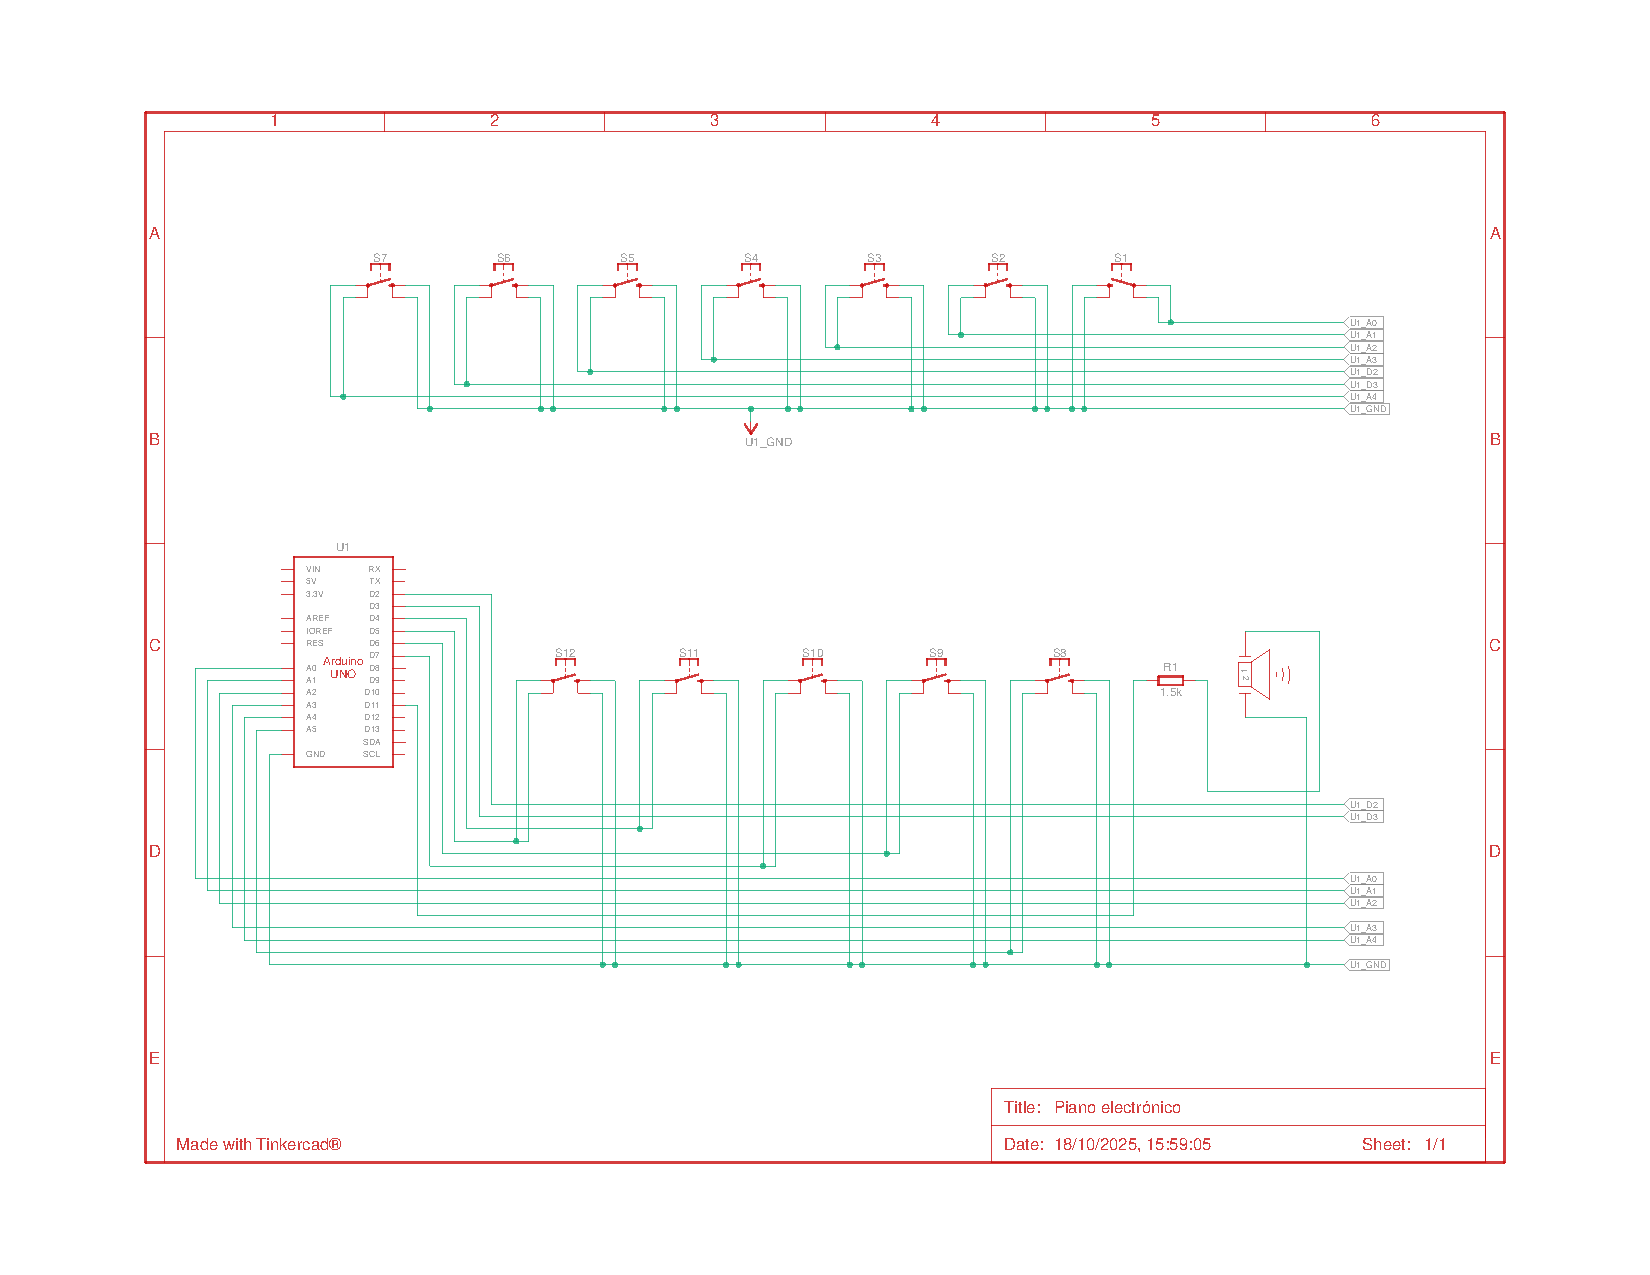
\includegraphics[width=0.5\textwidth]{Anexos/Conexionado_de_piano.pdf}
    \caption{Esquema de conexión del piano electrónico. Elavoración propia en Tinkercad®.}
    \label{fig:conexion_piano}
\end{figure}

\subsubsection{Cerradura electrónica}

En la Figura~\ref{fig:Cerradura_electronica} se presenta el esquema de conexión del sistema de cerradura electrónica. 
El circuito fue diseñado en Tinkercad® y muestra la interconexión entre el microcontrolador ATmega328P, el teclado matricial 4×4, 
la pantalla LCD 16×2 con interfaz I²C, los LEDs indicadores (rojo y verde) y el buzzer de señalización.

\begin{figure}[H]
    \centering
    \includegraphics[width=0.5\textwidth]{Anexos/Cerradura_electrónica.pdf}
    \caption{Esquema de conexión del candado electrónico. Elaboración propia en Tinkercad®.}
    \label{fig:Cerradura_electronica}
\end{figure}
